%TC:group tabular 1 1
%TC:group table 1 1

\chapter{Preparation}

\paragraph{} This chapter shall first address the refinements made to the project proposal. Then I shall explain the tests that established Excel's suitability for musical development. Next, the initial design decisions for Excello shall be explained. The software engineering tools and techniques employed will then be introduced. Finally, the research conducted to decide to implement the converter from MIDI to Excello shall be summarised.

\section{Proposal Refinements}

\paragraph{} The project designed a notation for defining music within a spreadsheet, along with a system for interpreting this to produce audio output. This continued to explore abstracting time away from the grid.

\paragraph{} This would be implemented as an Excel add-in subject to successful initial testing. An add-in is a web application displayed within Excel that can read and write to the spreadsheet using the Office Javascript API\footnote{https://docs.microsoft.com/en-us/javascript/api/excel?view=office-js}. Arbitrary additional data and markup can be included in the spreadsheet. Tests verified that audio output can be produced for music end-user music programming within Excel.

\paragraph{} A sizeable addition to the project beyond the initial proposal was to perform participatory design \cite{muller:pd} to advise on improvements beyond the initial prototype. Participants would be able to identify aspects of the current design that (don't) work well or add cognitive difficulty. This lead to the implementation of new features and improvements. As a result, the proposed extension of live-coding would only be implemented if deemed high priority by the participants. Participants who gained sufficient familiarity with the project were used for more informed summative evaluation.

\paragraph{} The converter translated MIDI to a CSV file for use with Excello. Explanation on the choice of MIDI is provided below. It was also motivated by participants who wished to integrate Excello with their use of digital audio workstations such as Logic Pro, Ableton Live, and GarageBand.

\section{Feasibility Analysis}

\paragraph{} The following section outlines the tests carried out to assess the feasibility of synthesising notes with data in a spreadsheet using an Excel add-in. All tests were carried out in Excel Online\footnote{https://office.live.com/start/Excel.aspx} using Script Lab\footnote{https://www.microsoft.com/en-us/garage/profiles/script-lab/}, an add-in that allows users to create and test simple add-ins experimenting with the Office Javascript API. These add-ins can access libraries and data elsewhere online.

\paragraph{} If add-ins were run in an older version of Internet Explorer, playing sound or using the Web Audio API would be possible.An add-in that played a WAV file verified that sound could be created. \cite{mozilla:webaudioapi}.

\subsection{Note Synthesis Library}

\paragraph{} The Web Audio API allows audio to be synthesised from the browser using Javascript \cite{mozilla:webaudioapi}. Creating a program for users to define and play musical structures requires synthesising arbitrary length, pitch and volume notes. To avoid the lower-level audio components (e.g. oscillators), I researched libraries that would allow me to deal with higher level musical abstractions of the synthesised notes. Sarkar's SheetMusic used the library tones\footnote{https://github.com/bit101/tones}, an API where only the pitch and volume envelope\footnote{How the note's volume changes over its duration} of the notes. This also only included simple waveform synthesisers.

\paragraph{} Tone.js\footnote{https://tonejs.github.io/} is a library built on top of the Web Audio API that provides greater functionality. An \texttt{Instrument} such as a \texttt{Synth} or \texttt{Sampler} is defined. The \texttt{triggerattackrelease} release method of these instruments allows a note of a given pitch, volume and duration to be triggered at a particular time. Notes are defined using scientific pitch notation (SPN) (e.g. \texttt{e.g. F\#4}), name (with accidental\footnote{Sharp or flat symbol used for black notes on a piano.} if required) (e.g. \texttt{F\#}) combined with octave (\texttt{4}). As Script Lab can reference libraries from the Node Package Manager (NPM), I tested playing notes with pitch defined in the add-in Javascript.

\subsection{Office Javascript API}

\paragraph{} To produce music within Excel, the musical output must be informed by the data in the spreadsheet. Previous tests defined notes in the add-in Javascript. To test the Excel API, I played a note with the pitch defined in the spreadsheet. This was extended so note playing, not just the pitch, was defined within a cell (\texttt{play(F\#4)}), detected and executed.

\paragraph{} Next, I was able to play a sequence of constant length notes defined in consecutive cells (\texttt{play(H1:K1)}). The range of cells was accessed using the Excel API and the values were played using the \texttt{Tone.Sequence} object. These tests confirmed Tone.js combined with the Excel API provided adequate functionality to implement the project as an add-in.

\section{Excello Design and Language}

\subsection{Abstracting Time}

\paragraph{} Dave Griffith's Al-Jazari \cite{mclean:visualisation} takes place in a three-dimensional world where robotic agents navigate around a two-dimensional grid. The height and colour of the blocks over which the agents traverse determines the sound they produce. The characteristics of the blocks are modified manually by users at run-time whilst the agents are moving. The basic instructions have the agents rotate and move forwards and backwards in the direction that they are facing. There exists a dual formalism in both the agent's instructions and the block state. This design is intended to improve live coding accessibility, both when viewing performances and becoming a live coder.

\begin{figure}[ht]
  \centerline{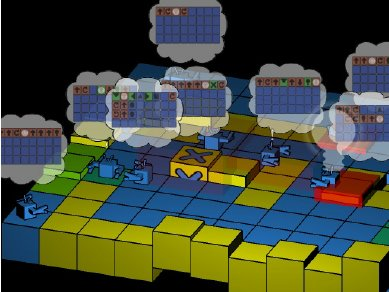
\includegraphics[width=100mm]{figs/alJazari.jpg}}
\caption{Programmed agents moving around a grid in Al-Jazari \textcopyright\ Alex Mclean}
\label{prep:alJazari}
\end{figure}

\vspace{-20pt}
\paragraph{} In Al-Jazari, the agents are programmed with symbols corresponding to different movements in thought bubbles above them. This is not suitable for programming within spreadsheets where all data must exist alphanumerically within cells. If an agent was to continue moving forwards many times in a row, it would become tiresome to keep adding this symbol. This is less of an issue in Al-Jazari where the grid only measures ten cells wide and long.

\paragraph{} Having a cursor navigate around a cartesian plane is the method used by turtle graphics. Just as this concept is used in Al-Jazari for agents to play the cell they occupy rather than colour it, it is suitable for spreadsheets. The turtle abstraction is employed by Excello by defining notes in cells and agents, known as turtles, to move through the spreadsheet activating them. To play a chord, multiple turtles must simultaneously pass through multiple cells corresponding to the notes of the chord. This maintains high notational consistency but sacrifices the abstractions for musical structures that are available in languages like Sonic Pi - \texttt{chord(\upquote{F\#}, \upquote{maj7})}. By implementing methods in the add-in to add the notes of chords to the grid, abstractions can be maintained whilst preserving consistency and cleanness in the spreadsheet itself.

\paragraph{} Turtle are the crux of the Logo programming language \cite{goldman:turtle} where turtles are programmed entirely by text to produce graphical output. For example, \texttt{repeat 4 [forward 5 right 90]} has a turtle move forwards 50 units and turn 90 degrees to the right four times to draw a square. A similar method is employed in Excello but the language is designed to be less verbose.

\subsection{Initial Prototype Design}

\paragraph{} Notes are placed in the cells of the spreadsheet and turtles are defined to move through the grid using a language based on Logo. The notes in cells are played when turtles move through those cell. When the play button is pressed, the melodic lines produced by all turtles defined in the grid are played concurrently. Turtles are defined with a start cell, movement instructions, the speed they move through the grid at (cells per minute) and the number of times they repeat their path. As in Al-Jazari, distance in space maps to time \cite{mclean:texture}. Excello extends upon this as turtles can move at different speeds. Therefore parts with longer notes can be defined more concisely and phase music\footnote{Music where identical parts are played at different speeds} can be easily defined. The Excello turtle movement instructions are explained below with examples.

\paragraph{} Turtles begin facing north. The move command, \texttt{m}, moves the turtle one cell forward. Like Logo, turtles always move in the direction they are facing. The commands \texttt{l} and \texttt{r} turn the turtle 90 degrees left and right respectively. Logo commands are repeated with \texttt{repeat} followed by the number of repeats and the commands \cite{goldman:turtle}. To reduce verbosity, single commands are repeated by placing a number immediately after it. For example, \texttt{m4} has the turtle move forwards four cells in the direction that it is facing. The direction a turtle is facing can be defined absolutely with \texttt{n}, \texttt{e}, \texttt{s} and \texttt{w} to face the turtle north, east, south and west. These rotate the turtles rather than moving them to maintain the consistency that turtles always move in the direction they face. To change notes' volume, dynamics (\texttt{ppp}, \texttt{pp}, \texttt{p}, \texttt{mp}, \texttt{mf}, \texttt{f}, \texttt{ff}, \texttt{fff}) can be placed within the turtle instructions. Any notes played after are played at that dynamic. Just as dynamics in western notation are a property of the staff, not individual notes, dynamics were originally defined in the turtle not notes. To repeat multiple instructions, they are placed in brackets followed by the number of repeats. For example, \texttt{(r m5)4}  defines a clockwise path around a five by five square. This seven character example is equivalent to the above Logo example which requires 29 characters. This repetition of instruction is why relative movements \texttt{l} and \texttt{r} are included in the language despite being less explicit than the compass based directions. This is demonstrated in figure \ref{prep:language1}.

\begin{figure}[ht]
  \centerline{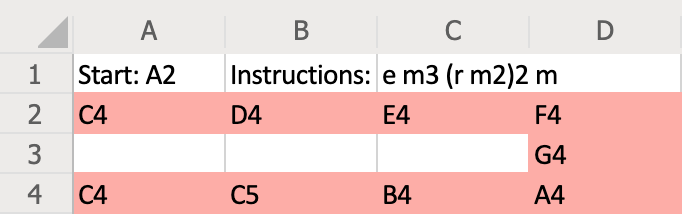
\includegraphics[width=100mm]{figs/diss1.png}}
\caption{The instructions for a turtle following the path of notes from A2 to A4}
\label{prep:language1}
\end{figure}

\paragraph{} It may not be convenient to constrain each melodic line to a single path of adjacent cells. Just as conventional score notation often spans across multiple lines, splitting up parts is a useful form of secondary notation. This requires the turtle to move to non-adjacent cells. For graphic drawing in Logo, lifting the pen allows the turtle to move without colouring the space beneath it. However, here the number of steps the turtle takes doesn't affect the output, only the cells it colours does. However, the musical output of Excello is dependent on the turtle's spacio-temporal information, so this would introduce large rests. Analogous to lifting the pen for graphical turtles, the turtle could enter a mode where it passes through cells immediately without playing them until it is placed back in playing mode. Here the actual path of the turtle is insignificant, only the cell it ends up in. I have therefore added jumps to the language. This can be defined with \texttt{j} in absolute terms with a destination cell (e.g. \texttt{jA5}), or relatively (e.g. \texttt{j-7+1}), with the number of rows and columns jumped. An absolute jump may be more explicit for human readers, but relative jumps facilitate repeats jumping to different cells each time. For example, \texttt{r (m7 j-7+1)9 m7} plays 10 rows of 8 cells from top to bottom playing each row left to right. A jump is demonstrated in figure \ref{prep:language2}.

\begin{figure}[ht]
  \centerline{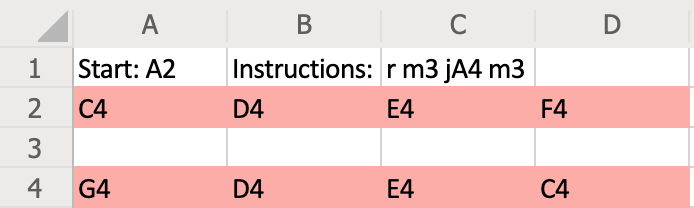
\includegraphics[width=100mm]{figs/diss2.png}}
\caption{The instructions for the path from A2 to D2 then A4 to D4}
\label{prep:language2}
\end{figure}
\vspace{-20pt}

\paragraph{} The language for turtle movement instructions is summarised by the following context-free grammar, $(N,\Sigma,S,\mathcal{P})$. Non-terminal symbols $N=(\langle$Full Instructions$\rangle, \langle$Instruction Series$\rangle, \langle$Single Block$\rangle, \langle$Command$\rangle, \langle$Relative$\rangle, \langle$Absolute$\rangle, \langle$Sign$\rangle, \langle$Cell$\rangle, \langle$Dynamic $\rangle)$, terminal symbols $\Sigma=(z{\in}\mathbb{Z}, n{\in}\mathbb{N}, c{\in}\texttt{[A-Za-z]}^{+}, \texttt{m}, \texttt{j}, \texttt{l}, \texttt{r}, \texttt{n}, \texttt{e}, \texttt{s}, \texttt{w}, \texttt{+}, \texttt{-}, \texttt{ppp}, \texttt{pp}, \texttt{p}, \texttt{mp}, \texttt{mf}, \texttt{f}, \texttt{ff}, \texttt{fff})$ and starting symbol $S = \langle \text{Full Instructions} \rangle$. The set of grammar rules $\mathcal{P}$ are shown in figure \ref{fig:grammar}:

% \begin{table}
% \centering
% % \caption{Grammar Rules for the turtle movement instructions. $z \in \Z$}
% \caption{Grammar rules for turtle movement instructions. $z \in \mathbb{Z}, n \in \mathbb{N}, c \in \texttt{[A-Za-z]}^{+}$.}
% \vspace{1pt}
% \begin{tabular}{|l|l|} \hline
% \textbf{Grammar Rule}&\textbf{Left Symbol Interpretation}\\ \hline
% \( \mathbf{S} \rightarrow \mathbf{Y} \)& Starting symbol\\ \hline
% \( \mathbf{Y} \rightarrow \mathbf{X} | \mathbf{X} \ \mathbf{Y} \)& A series of instructions\\ \hline
% \( \mathbf{X} \rightarrow (\mathbf{Y})z|\mathbf{I} \)& A single command or bracketed series of instructions\\ \hline
% \( \mathbf{I} \rightarrow \texttt{m}z|\mathbf{R}|\mathbf{R}z|\mathbf{A}|\mathbf{D}|\texttt{j}\mathbf{C}|\texttt{j}\mathbf{P}n\mathbf{P}n \)& A single command\\ \hline
% \( \mathbf{R} \rightarrow \texttt{l}|\texttt{r} \)& Relative rotation\\ \hline
% \( \mathbf{A} \rightarrow \texttt{n}|\texttt{e}|\texttt{s}|\texttt{w} \)& Absolute rotation\\ \hline
% \( \mathbf{P} \rightarrow \texttt{+}|\texttt{-} \)& Sign\\ \hline
% \( \mathbf{C} \rightarrow cz \)& Cell reference\\ \hline
% \( \mathbf{D} \rightarrow \texttt{ppp}|\texttt{pp}|\texttt{p}|\texttt{mp}|\texttt{mf}|\texttt{f}|\texttt{ff}|\texttt{fff} \)& Dynamic\\
% \hline\end{tabular}
% \label{tab:grammar}
% \end{table}

% \setlength{\grammarindent}{11em}
% \setlength{\grammarparsep}{2pt}
% \begin{figure}[ht]
%   \begin{grammar}
%       <Full Instructions> ::= <Instruction Series>
%
%       <Instruction Series> ::= <Single Block> | <Single Block><Instruction Series>
%
%       <Single Block> ::= (<Instruction Series>)$n$ | <Command>
%
%       <Command> ::= m$z$ | <Relative> | <Relative>$z$ | <Absolute> | <Dynamic> | j<Cell>
%       \alt j<Sign>$n$<Sign>$n$
%
%       <Relative> ::= l | r
%
%       <Absolute> ::= n | e | s | w
%
%       <Sign> ::= + | -
%
%       <Cell> ::= $cz$
%
%       <Dynamic> ::= ppp | pp | p | mp | mf | f | ff | fff
%   \end{grammar}
%   \vspace{-10pt}
% \caption{The grammar of the turtle movement instructions in Backus-Nour form}
% \label{fig:grammar}
% \end{figure}

\newenvironment{bnfsplit}[1][0.7\textwidth]
 {\minipage[t]{#1}$}
 {$\endminipage}

\begin{figure}[ht]
\renewcommand{\models}{::=}
\begin{bnf*}
  \bnfprod{Full Instructions}
  {
  \bnfpn{Instruction Series}
   }\\
  \bnfprod{Instruction Series}
    {
    \bnfpn{Single Block}
    \bnfor \bnfpn{Single Block}\bnfpn{Instruction Series}
     }\\
 \bnfprod{Single Block}
   {
   \texttt{(}\bnfpn{Instruction Series}\texttt{)}n
   \bnfor \bnfpn{Command}
    }\\
  \bnfprod{Command}
    {
    \begin{bnfsplit}
    \texttt{m}z
    \bnfor \bnfpn{Relative}
    \bnfor \bnfpn{Relative}z
    \bnfor \bnfpn{Absolute}
    \bnfor \bnfpn{Dynamic}
    \\ \bnfor \texttt{j}\bnfpn{Cell}
    \bnfor \texttt{j}\bnfpn{Sign}n\bnfpn{Sign}n
    \end{bnfsplit}
     }\\
   \bnfprod{Relative}
     {
     \texttt{l}
     \bnfor \texttt{r}
      }\\
  \bnfprod{Movement}
    {
    \texttt{n}
    \bnfor \texttt{e}
    \bnfor \texttt{s}
    \bnfor \texttt{w}
     }\\
 \bnfprod{Sign}
   {
   \texttt{+}
   \bnfor \texttt{-}
    }\\
  \bnfprod{Cell}
    {
    cz
     }\\
 \bnfprod{Dynamic}
   {
   \texttt{ppp}
   \bnfor \texttt{pp}
   \bnfor \texttt{p}
   \bnfor \texttt{mp}
   \bnfor \texttt{mf}
   \bnfor \texttt{f}
   \bnfor \texttt{ff}
   \bnfor \texttt{fff}
    }\\
\end{bnf*}
\vspace{-35pt}
\caption{The grammar rules, $\mathcal{P}$, for turtle movement instructions in Backus-Nour form}
\label{fig:grammar}
\end{figure}

\paragraph{} Notes are defined in the cells using SPN. Empty cells are interpreted as rests. To create notes longer than a single cell, the character \texttt{s} sustains the note that came before it as in figure \ref{prep:sustainMulti} (a). A cell can be subdivided time-wise into multiple notes with multiple comma separated notes as in figure \ref{prep:sustainMulti} (b). This was designed so the length a cell corresponds to is not bound by the length of the smallest note in the piece. For example, a piece defined primarily with crotchets (one unit) but with occasional quavers (half a unit) does not necessitate double the number of cells and introduce many additional \texttt{s} cells in the entire piece.

\begin{figure}[ht]
\begin{tabular}{cc}
  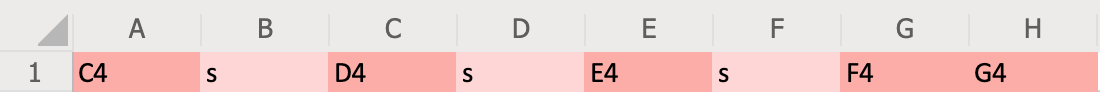
\includegraphics[height=8mm]{figs/withoutMulti.png} &
  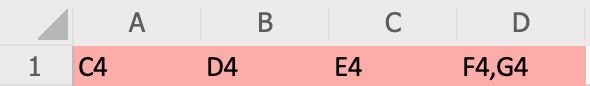
\includegraphics[height=8mm]{figs/withMulti.png} \\
  (a) Using sustain cells&(b) Using a multi-note cell\\
\end{tabular}
\caption{Two identical motifs defined by using sustains or with multi-note cells}
\label{prep:sustainMulti}
\end{figure}

\section{Software Engineering}

\subsection{Requirements}

\paragraph{} The success criteria of the project are:

\begin{enumerate}
  \item Implementation of an system for music playback within a spreadsheet where users can:
  \begin{itemize}
     \item Play individual notes and chords with defind durations.
     \item Define multiple parts.
     \item Play loops.
     \item Define sequences of notes and chords and be able to call these for playback.
     \item Define the tempo of playback.
   \end{itemize}
  \item Participatory design with formative evaluation sessions.
  \item Summative evaluation with participants who have gained familiarity with the system.
  \item Implementation of a converter from MIDI to the spreadsheet representation.
  \item In addition to these, the following extension work was completed:
  \begin{itemize}
     \item Implement additional features that arise from participatory design.
     \item Explore a compressive conversion from MIDI to the Excel system.
   \end{itemize}
\end{enumerate}

\subsection{Tools and Technologies Used}

Table \ref{intro:tools} outlines the tools, languages and libraries used.

\begin{table}[ht]
\centering
\vspace{1pt}
\begin{tabular}{|l|l|l|} \hline
\textbf{Software}&\textbf{Type}&\textbf{Usage}\\ \hline
Scriptlab&Add-in&Writing initial Excel add-in tests. \\ \hline
Typescript&Language&Writing Excello. Used for static type\\
&&checking and Javascript libraries. \\ \hline
Yeoman\tablefootnote{A generator for scaffolding Node.js web applications, https://github.com/OfficeDev/generator-office}&Add-in Generator&Creating the blank Excel add-in project.\\ \hline
NodeJS&Javascript&Manage library dependecies and run local web\\
&Environment&servers. \\ \hline
Surge\tablefootnote{Static webpage publishing tool and hosting https://surge.sh/}&CDN&Hosting Excello online for participants' use.\\ \hline
Jupyter&Python&Implementing the MIDI to Excello converter.\\ Notebook&Environment& \\ \hline
Tone.js&Library&Synthesising and scheduling sound via the Web\\
&&Audio API.\\ \hline
tonal&Library&Generating the notes of chords.\\ \hline
Mido\tablefootnote{https://mido.readthedocs.io/en/latest/}&Library&Reading MIDI files in Python.\\ \hline
\end{tabular}
\caption{Tools used during the project}
\label{intro:tools}
\end{table}

% \paragraph{} Initial tests were written in Javascript in the Script Lab add-in for Excel. Excello was written in Typescript as this is readily compiled into the Javascript required to run the add-in but provides static type-checking. It also allows the large collection of existing Javascript libraries to be utilised. Using the Yeoman generator\footnote{A tool for scaffolding Node.js web applications, https://github.com/OfficeDev/generator-office} I created a blank Excel add-in project. I used NodeJS to manage dependencies to other Javascript libraries. During development, I ran the add-in on localhost. To allow participants to run Excello on their own machines, I hosted a version of the add-in online using Surge\footnote{Static webpage publishing tool and hosting https://surge.sh/}. To run the add-in in Excel, a manifest.xml file is imported which instructs Excel where the add-in is hosted. The converter from MIDI to Excello was implemented in Python using Jupyter Notebooks.
%
% \paragraph{} The Tone.js library was used to synthesise and schedule sound production via the Web Audio API. The Javascript music theory library tonal was used to produce the notes of chords. This prevented the hardcoding of the intervals present in the 109 chords available. The Python library Mido was employed to read python files. All of these libraries have an MIT license. I used the Salamander Grand Piano V3\footnote{https://freepats.zenvoid.org/Piano/acoustic-grand-piano.html} sample pack in order to synthesise realistic piano playback. This is under the creative commons liscence\footnote{http://creativecommons.org/licenses/by/3.0/}
%
\subsection{Starting Point}

\paragraph{} Having used the Yeoman generator to create an empty Excel add-in, all the code to produce Excello and the MIDI converter was produced from scratch using the libraries described above.

\paragraph{} I had written simple Javascript for small websites, but had no experience using Node, libraries or building a larger project. Having never used any of the libraries before, reviewing the documentation was required before and during development. I had gained experience with Python and Jupyter Notebooks from a summer internship.

\subsection{Evaluation Practices}

\paragraph{} To best tune Excello's to the needs of potential users, formative evaluation sessions were carried out with participants. A spiral development methodology \cite{boehm:spiral} was used. This iterates the following steps: determining objectives, identify problems and solutions, develop and test, deploy and prepare next iteration. This was more suitable than sequential document-driven process methods such as the waterfall method. Due to the number of participants and the project timeframe, there were only two major development iterations with additional incremental updates. The first prototype, and the second fixing issues and implementing requests from participants.

\paragraph{} Summative evaluation was carried out with users involved in participatory design. Therefore, experienced users of Excello could be used for evaluation despite the product not yet being released in the public domain.

\section{MIDI files}

\paragraph{} MIDI is a communications protocol to connect electronic musical instruments with devices for playing, editing and recording music. A MIDI file consists of event messages describing on/off triggerings to control audio \cite{huber:midimanual}. MIDI files were designed to be produced by MIDI controllers such as electric keyboards. As such, MIDI files contain controller specific information that is not necessary for the creation of an Excello file. Musical formats such as MusicXML specify the musical notation and could be suitable for conversion to Excello.

\paragraph{} Many programs support importing and exporting MIDI files. By converting MIDI files to the Excello notation, Excello is more integrated into the environment of programs for playing, editing and composing music. Furthermore, there exist many datasets available for MIDI \cite{huang:deep} which can immediately be played back for comparison.
